% 第4章 前期基础工作

\chapter{四、前期基础工作}

\section{1）结构设计}

a. 中红外 QCL-TDLAS 折返式长光程原位测量光路（含原位反射框架制作）如图 4 所示。四通道中红外 QCL 激光器与中红外探测器布置在试验段的同一侧，激光经试验段两侧壁面反射镜组在流场中多次折返后由探测器接收，气流穿过光路区。折返式（多程）结构在不加大装置尺寸的前提下把有效吸收光程提高数倍，使 ppm 量级 NO 的积分吸光度由``难以分辨''提升到``可稳定反演''；多程光路被约束在同一测量截面附近，与下游 PLIF 面测量处于同一测量区域，为两种手段的交叉校验提供几何一致性。该部分的具体研究内容包括反射镜组排布与光轴对准（即原位反射框架的制作与装调）、有效光程长度标定、窗口污染引起的透过率漂移补偿，以及激光光束抖动对反演稳定性的影响。

\begin{figure}[H]
  \centering
  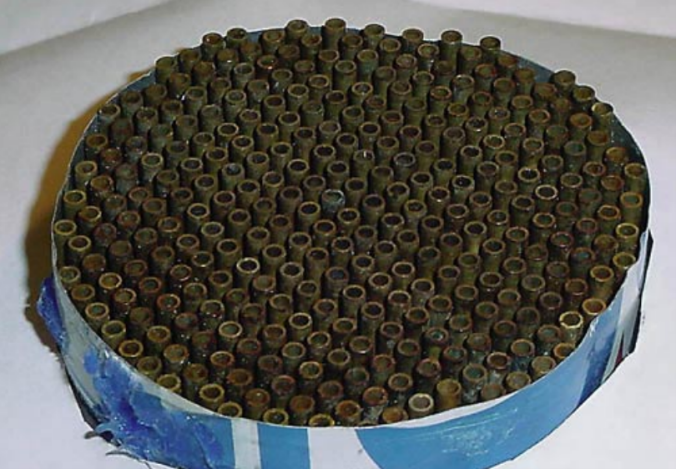
\includegraphics[width=0.85\textwidth]{figures/image4.png}
  \caption{原位测量试验台}
  \label{fig:test-rig}
\end{figure}

b. 染料激光光路与高压染料循环/蓄能缓冲系统（含染料循环泵系统制作）如图 5—8 所示。Nd:YAG 泵浦激光输出 1064 nm 基频，经 KTP 晶体倍频产生 532 nm 绿光，二向色镜滤除残余 1064 nm 后，由 $\lambda/2$ 半波片与格兰棱镜调节偏振态与能量，再经转向镜与聚光透镜耦合进入 Rh6G 染料池；染料激光在``扩束型光栅 + 输出耦合镜''构成的振荡腔内实现 560--650 nm 连续可调谐输出，最后经 BBO 晶体倍频、Pellin-Broca 棱镜分光，得到 283 nm 紫外输出。

\begin{figure}[H]
  \centering
  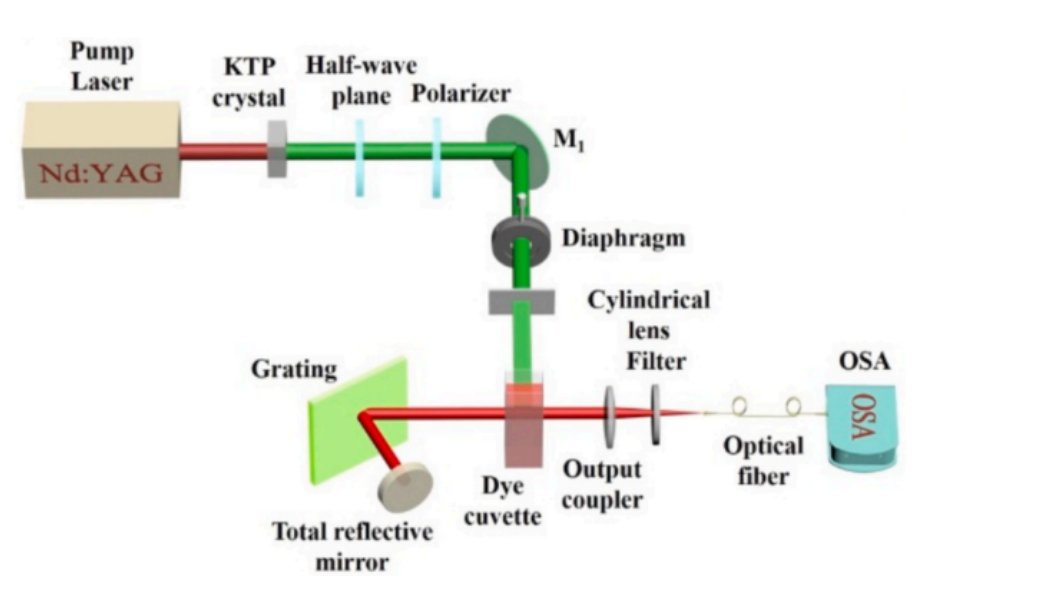
\includegraphics[width=0.75\textwidth]{figures/image5.png}
  \caption{染料激光工作示意图}
  \label{fig:dye-schematic}
\end{figure}

\begin{figure}[H]
  \centering
  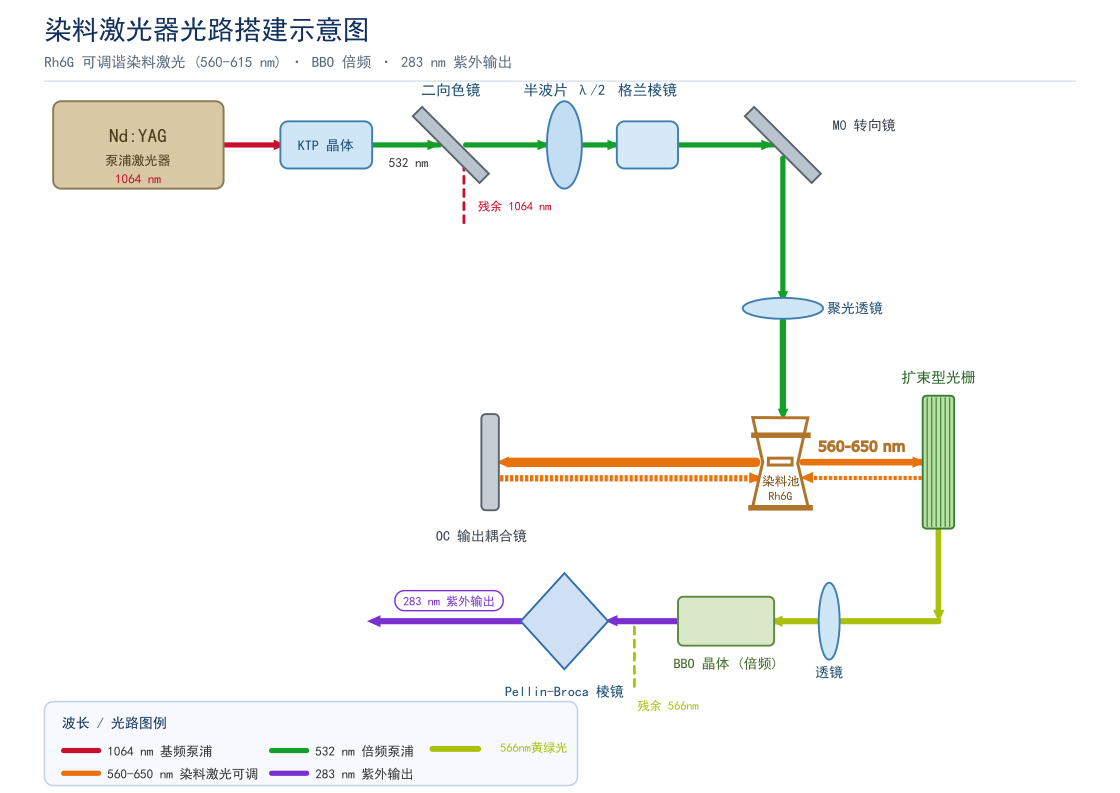
\includegraphics[width=0.85\textwidth]{figures/image6.png}
  \caption{染料激光器光路搭建示意图}
  \label{fig:dye-optical-path}
\end{figure}

高重频下染料池内的热积累与汽蚀是光束质量退化的主控因素，为此设计高压染料循环与蓄能缓冲系统（染料循环泵系统制作）如图 7 所示，是系统整体示意图。图 8 所示是染料泵装置实物图：介质罐中的染料经球阀、齿轮泵/柱塞泵、单向阀与针阀进入液压缸，再经三路单向阀与观察窗回流至泵前构成闭式循环；氮气瓶经减压阀、高压球阀与控压针阀向液压缸加压，形成增压与蓄能缓冲支路，以高压蓄能缓冲抑制汽蚀、稳定流场，把高重频下的能量抖动与波前畸变控制在可接受范围内。回路中布置压力传感器、压力表与观察窗用于实时监测染料压力与流场脉动，气动电磁阀与安全阀承担快速卸压与超压保护功能。

\begin{figure}[H]
  \centering
  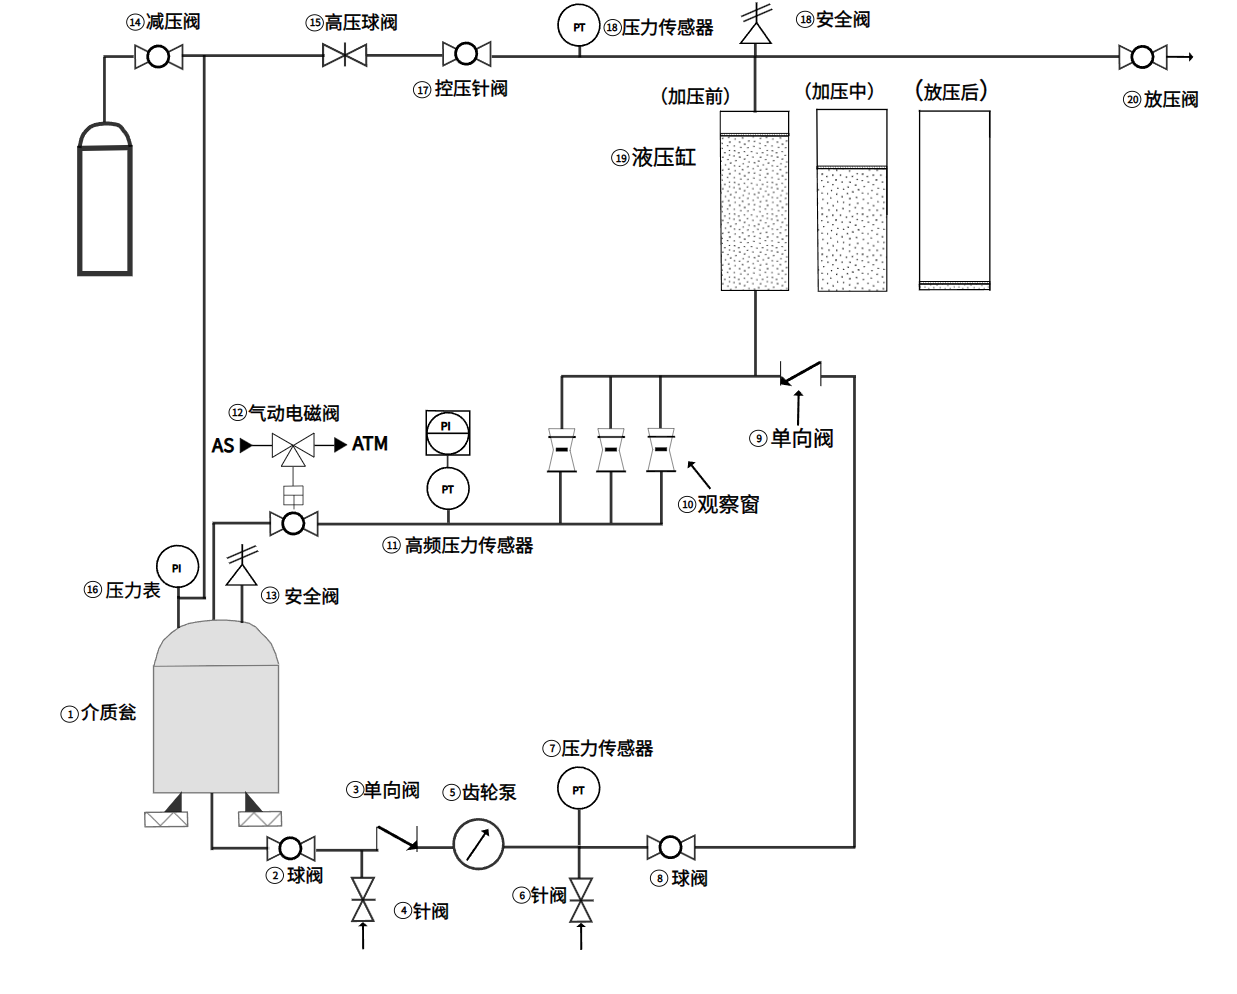
\includegraphics[width=0.85\textwidth]{figures/image7.png}
  \caption{染料泵循环系统示意图}
  \label{fig:dye-pump-system}
\end{figure}

\begin{figure}[H]
  \centering
  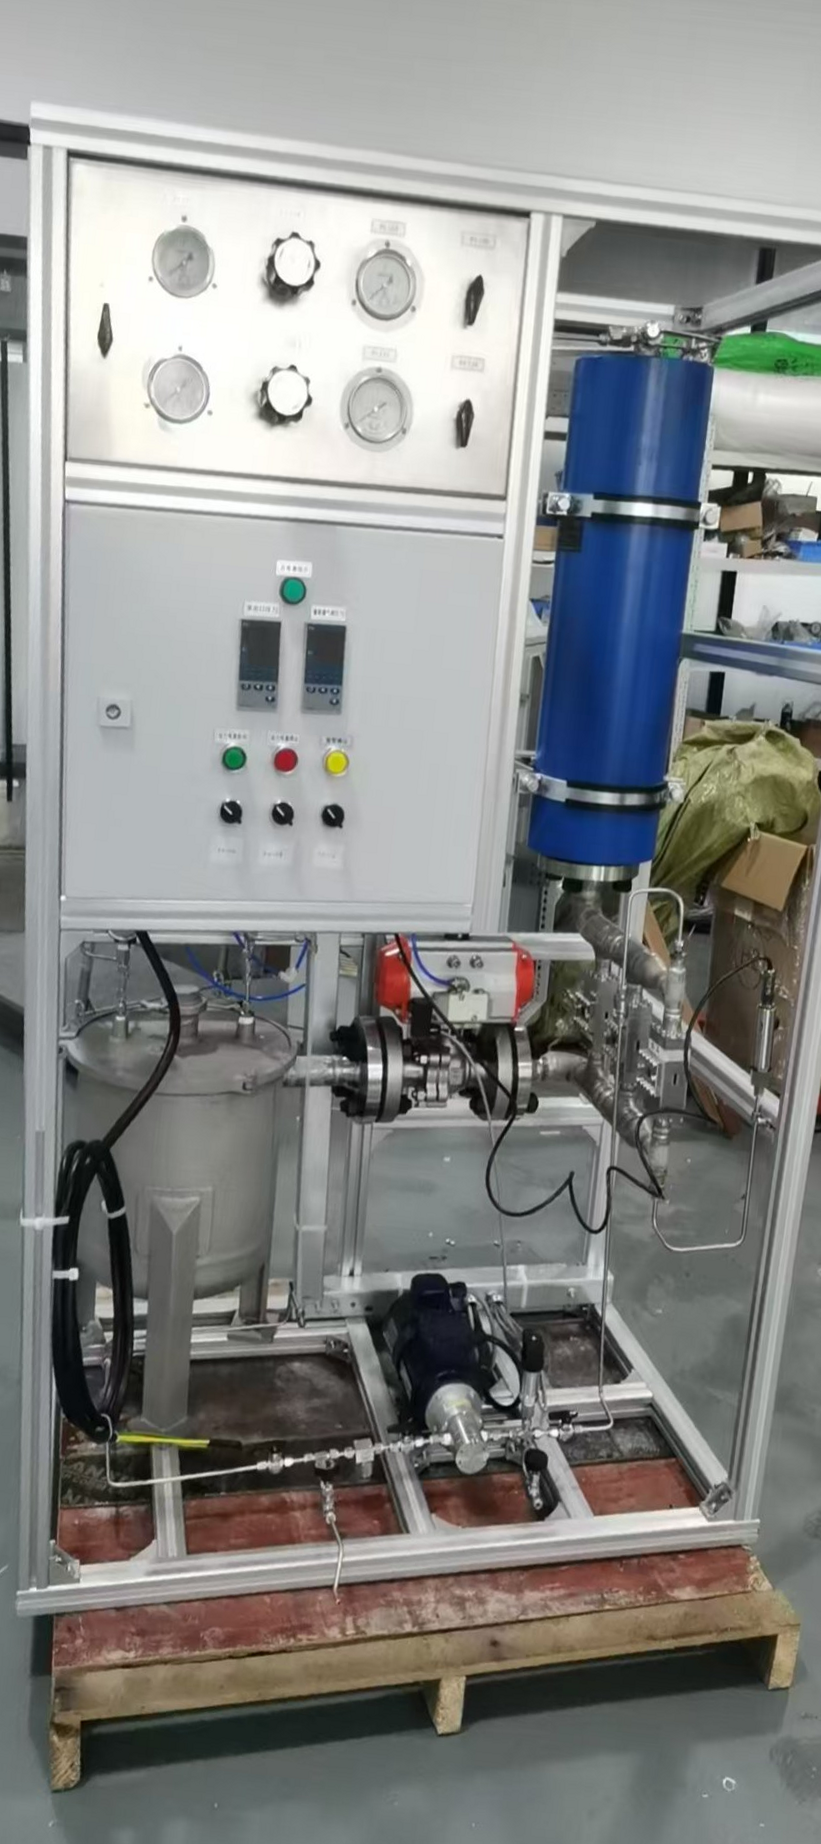
\includegraphics[width=0.35\textwidth]{figures/image8.png}
  \caption{染料泵装置实物图}
  \label{fig:dye-pump-photo}
\end{figure}

\section{2）试验研究}

a. 中红外 QCL-TDLAS 多组分在线测量试验。基于 HITRAN/HITEMP 数据库与自编 Voigt 线型程序，为目标工况优选 NO（5.2 μm）谱线，确保通道正常正常工作；搭建中红外 QCL 发射—探测系统，开展波长扫描与``吸收谱—温度—浓度''联合反演算法研究；结合 Cantera 一维火焰仿真完成测量结果的浓度/温度标定与误差评估。

如图 9 所示的是常见的空气常见的集中气体分子在不同温度下的吸收表现，图 10 则是 NO 在不同温度下的吸收表现。在 NO 探测波长的选取上，本文以其振转基频带（$v = 1 \leftarrow 0$，X$^2\Pi$，中心波数约 1876 cm$^{-1}$）所在的中红外 5.2--5.3 μm 区域为基础，多组分光谱仿真结果，将 NO 探测窗口选定为 1894--1914 cm$^{-1}$，主要依据如下：其一，该窗口覆盖 NO 基频带 R 支中段（R(4)--R(10) 附近），谱线强度位居整个谱带前列，吸光度充足且可选谱线数量多，便于筛选低干扰目标线；其二，由光谱仿真可见，CO$_2$ 与 CO 的吸收集中于 1894--1904 cm$^{-1}$，而 1900--1910 cm$^{-1}$ 附近 H$_2$O 谱线密度显著降低，NO 吸收在该子区间占主导，且窗口上沿之外（$>$1914 cm$^{-1}$）H$_2$O 谱线重新变得密集，故该窗口是保证 NO 线强度前提下干扰最小的折中选择；其三，该窗口在 300--1300 K 全温区范围内均保持可观的 NO 吸收强度，兼顾常温标定与高温燃烧在线测量需求，并可在同一窗口内选取两条低态能量不同的谱线实现双线法测温；其四，5.2--5.3 μm 波段光源（DFB-QCL、OPO 等）与探测器（热电制冷 MCT、VIGO 光伏探测器等）技术成熟，无紫外波段的深紫外光源损伤风险、火焰化学发光与强散射背景，并与课题组既有中红外吸收光谱探测体系兼容。综上，1894--1914 cm$^{-1}$ 是兼顾谱线强度、干扰水平、温度适应性与工程可实现性的 NO 优选探测窗口。

\begin{figure}[H]
  \centering
  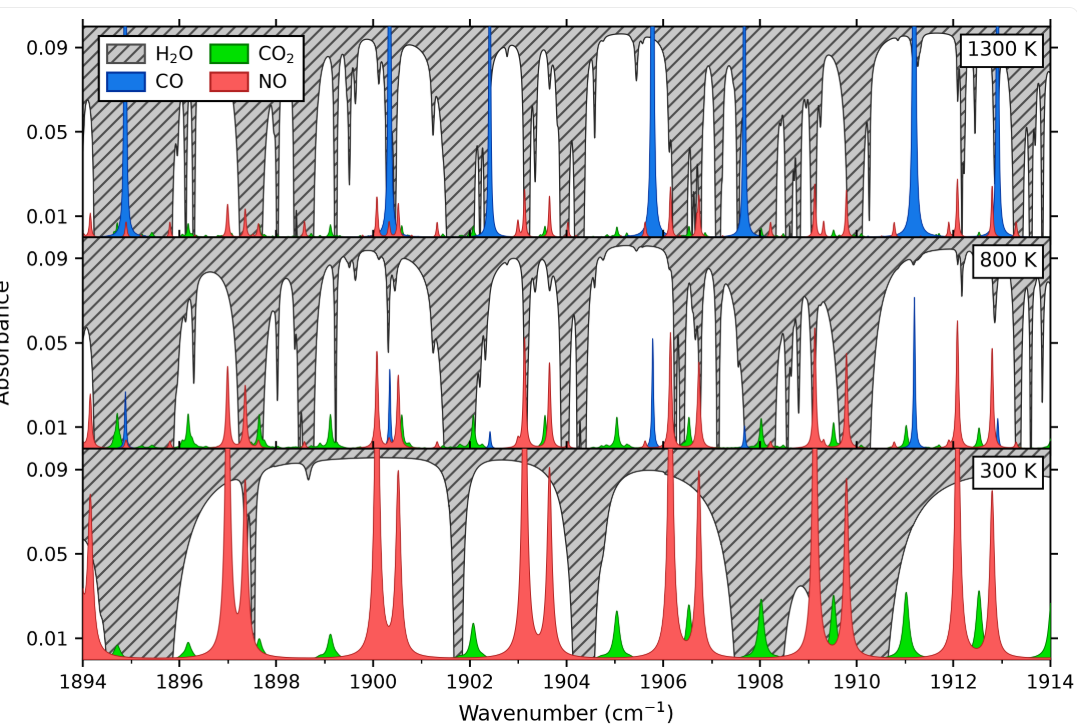
\includegraphics[width=0.85\textwidth]{figures/image9.png}
  \caption{四组分中红外吸收光谱温度特性（300 / 800 / 1300 K）}
  \label{fig:four-species-temp}
\end{figure}

\begin{figure}[H]
  \centering
  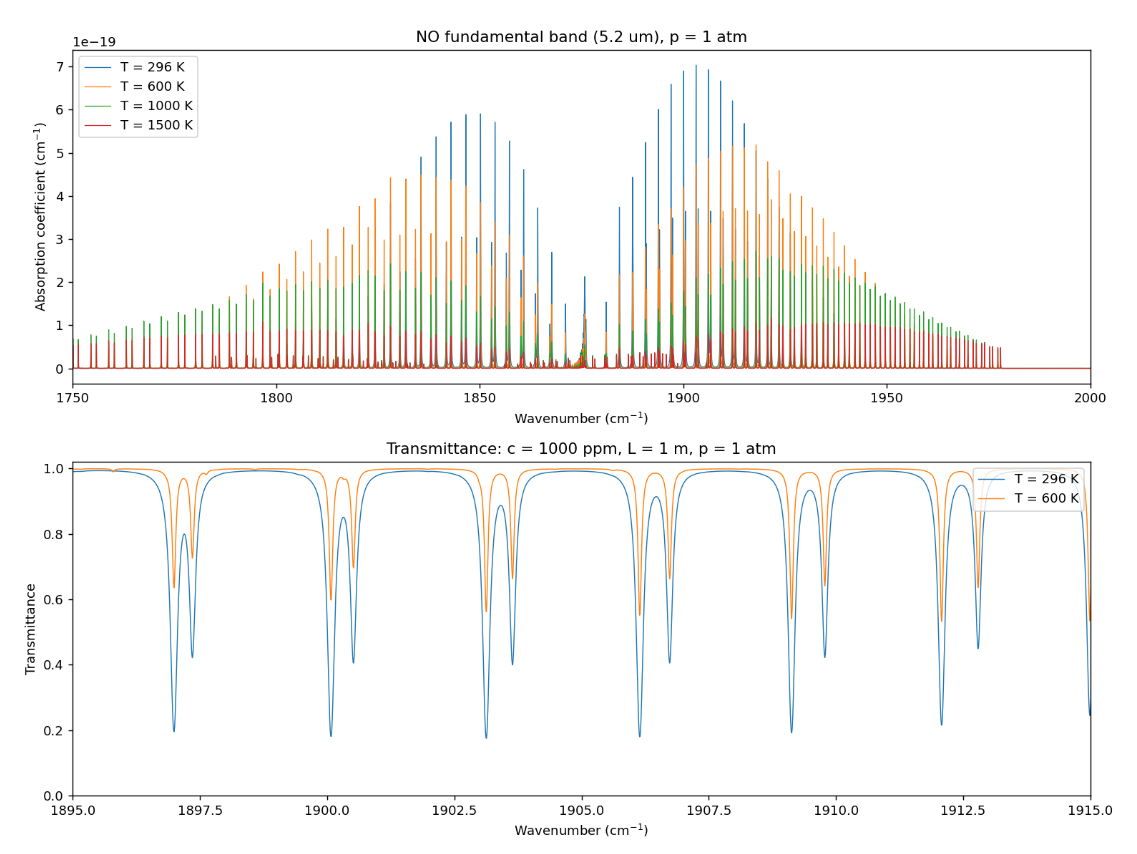
\includegraphics[width=0.8\textwidth]{figures/image10.png}
  \caption{NO 红外吸收光谱温度特性（1750--2000 cm$^{-1}$）}
  \label{fig:no-temp}
\end{figure}

\begin{figure}[H]
  \centering
  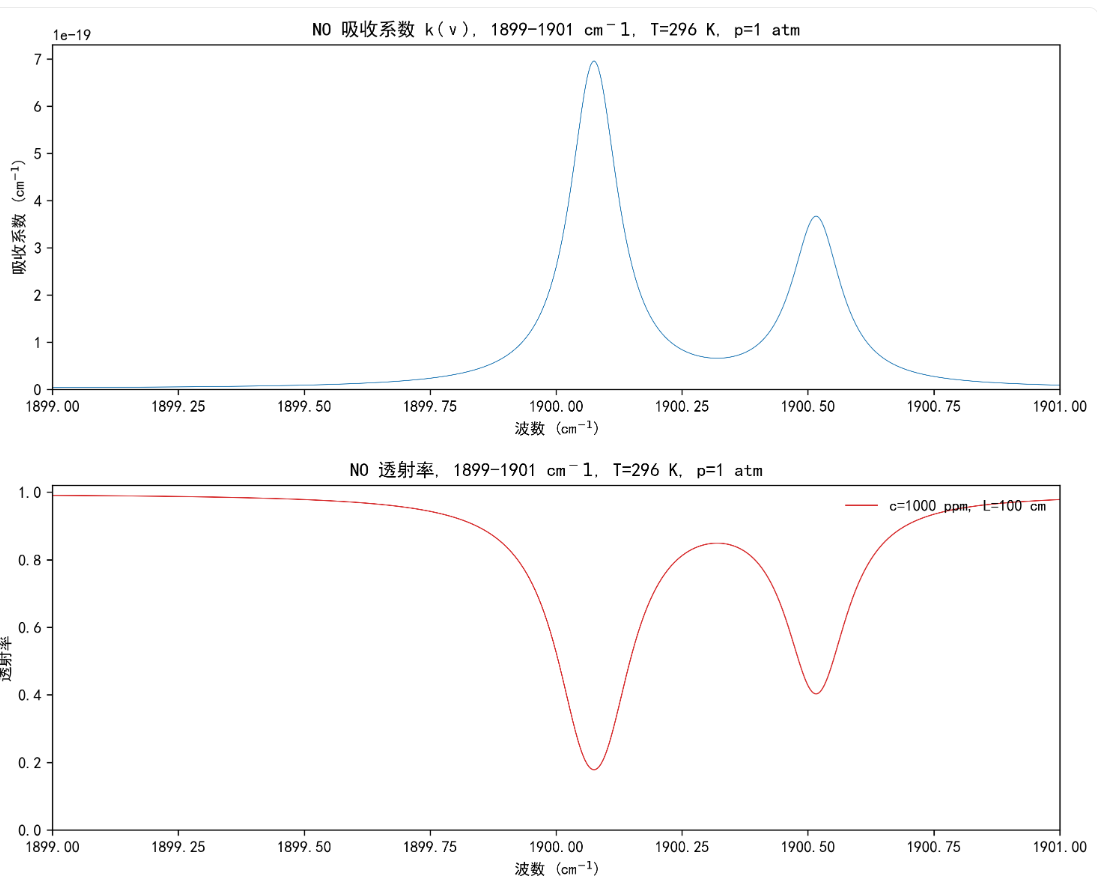
\includegraphics[width=0.8\textwidth]{figures/image11.png}
  \caption{NO 在 1900 cm$^{-1}$ 的吸收系数及透射率}
  \label{fig:no-1900}
\end{figure}

如图 11 所示，为 NO 在 1899--1901 cm$^{-1}$ 窄波段的吸收特性仿真结果。上图为该波段的吸收系数 $k(\nu)$ 分布，下图为对应典型测量工况（$c$ = 1000 ppm，$L$ = 100 cm，$T$ = 296 K，$p$ = 1 atm）下的透过率谱，两图横轴一致，分别反映谱线的固有吸收强度与实际可测信号。

由吸收系数谱可见，该波段内存在两条彼此分离的强吸收线，分别位于 1900.08 cm$^{-1}$ 与 1900.50 cm$^{-1}$。谱线呈典型 Lorentz 线型：296 K、1 atm 下多普勒展宽仅约 0.004 cm$^{-1}$，远小于压力展宽，Voigt 线型可近似为 Lorentz 线型；谱线半高全宽约 0.2 cm$^{-1}$，两线间距 0.42 cm$^{-1}$ 大于谱线半宽，因此可清晰分辨，但线翼仍存在一定重叠，定量反演时需考虑两线的相互贡献。

由透过率谱可见，在 1000 ppm 浓度、100 cm 光程条件下，两条谱线中心的透过率分别降至约 21\% 与 42\%，对应吸光度（$A = -\ln T$）约 1.56 与 0.87。这表明所选谱线在典型燃烧场浓度与光程条件下具有充足的吸收深度，可为直接吸收光谱或波长调制光谱测量提供足够的信噪比；同时也说明在 1000 ppm 高浓度工况下吸收已接近饱和区（$A > 1$）。

综上，该窄波段仿真验证了前文谱线优选的结果：上述两条强线位于 1900 cm$^{-1}$ 附近 H$_2$O 干扰相对最弱的区间，吸收深度适中，可作为 NO 浓度反演的目标谱线。

b. 高频 burst 染料激光 OH/NO-PLIF 成像试验。构建 burst 脉冲串泵浦的片光成像光路，配合高速相机开展 OH/NO-PLIF 二维瞬态测量；研究 burst 模式下染料激光输出稳定性（能量抖动、线宽展宽、波长漂移）及其对 PLIF 信号定量性的影响；以 283 nm 紫外片光照射测量区，由高速相机配合门控增强与窄带滤光采集 NO 荧光图像，开展``荧光强度—NO 浓度—温度/组分''的标定实验，评估碰撞猝灭与片光能量分布对信号定量性的影响，最终给出瞬态、高帧频的 NO 二维浓度场结果；通过切换激发波长，还可在同一切片下同步获取 OH 分布。

c. 点—面协同诊断与交叉校验试验。以统一的主时钟/触发源同步 QCL 波长扫描时序、burst 染料激光脉冲串与高速相机曝光时序，使 TDLAS 的单次光谱扫描与 PLIF 的脉冲串落在同一时间窗内；利用多程吸收光路与片光在试验段内的空间关系，把 TDLAS 的路径积分浓度映射到 PLIF 的二维浓度场上，由 PLIF 给出浓度不均匀度、构造路径积分权重、校正``路径平均浓度''与``峰值浓度''差异，反向以 TDLAS 免标定绝对浓度结果为 PLIF 标定提供基准，形成双向互校验；在 Hencken 标准火焰等可控工况下建立互校验模型与不确定度框架，随后在地面试验台/发动机尾气工况下验证适用性。
